\chapter{Metallurgie}	


\section{Metallurgie Titanlegierungen}
\section{Ti-6242}

Ti-6242 oder Ti-6Al-2Sn-4Zr-2Mo ist eine Alpha-Beta Titanlegierung, die  in 1967 eingeführt wurde.
Wie es im Phasendiagramm in Abbildung 1 zu erkennen ist, hat die Legierung Ti6242 bei Raumtemperatur ein hohes Alphaanteil und wird auch deshalb oft als eine Near-Alpha-Titanlegierung bezeichnet.

Neben Titan werden bei Ti6242 andere Legierungselemente zulegiert, um bestimmte Eigenschaften zu erreichen. Woraus die Ti-6242 besteht, ist in der Tabelle 1 abzulesen.


\begin{figure}[H]
	\centering
	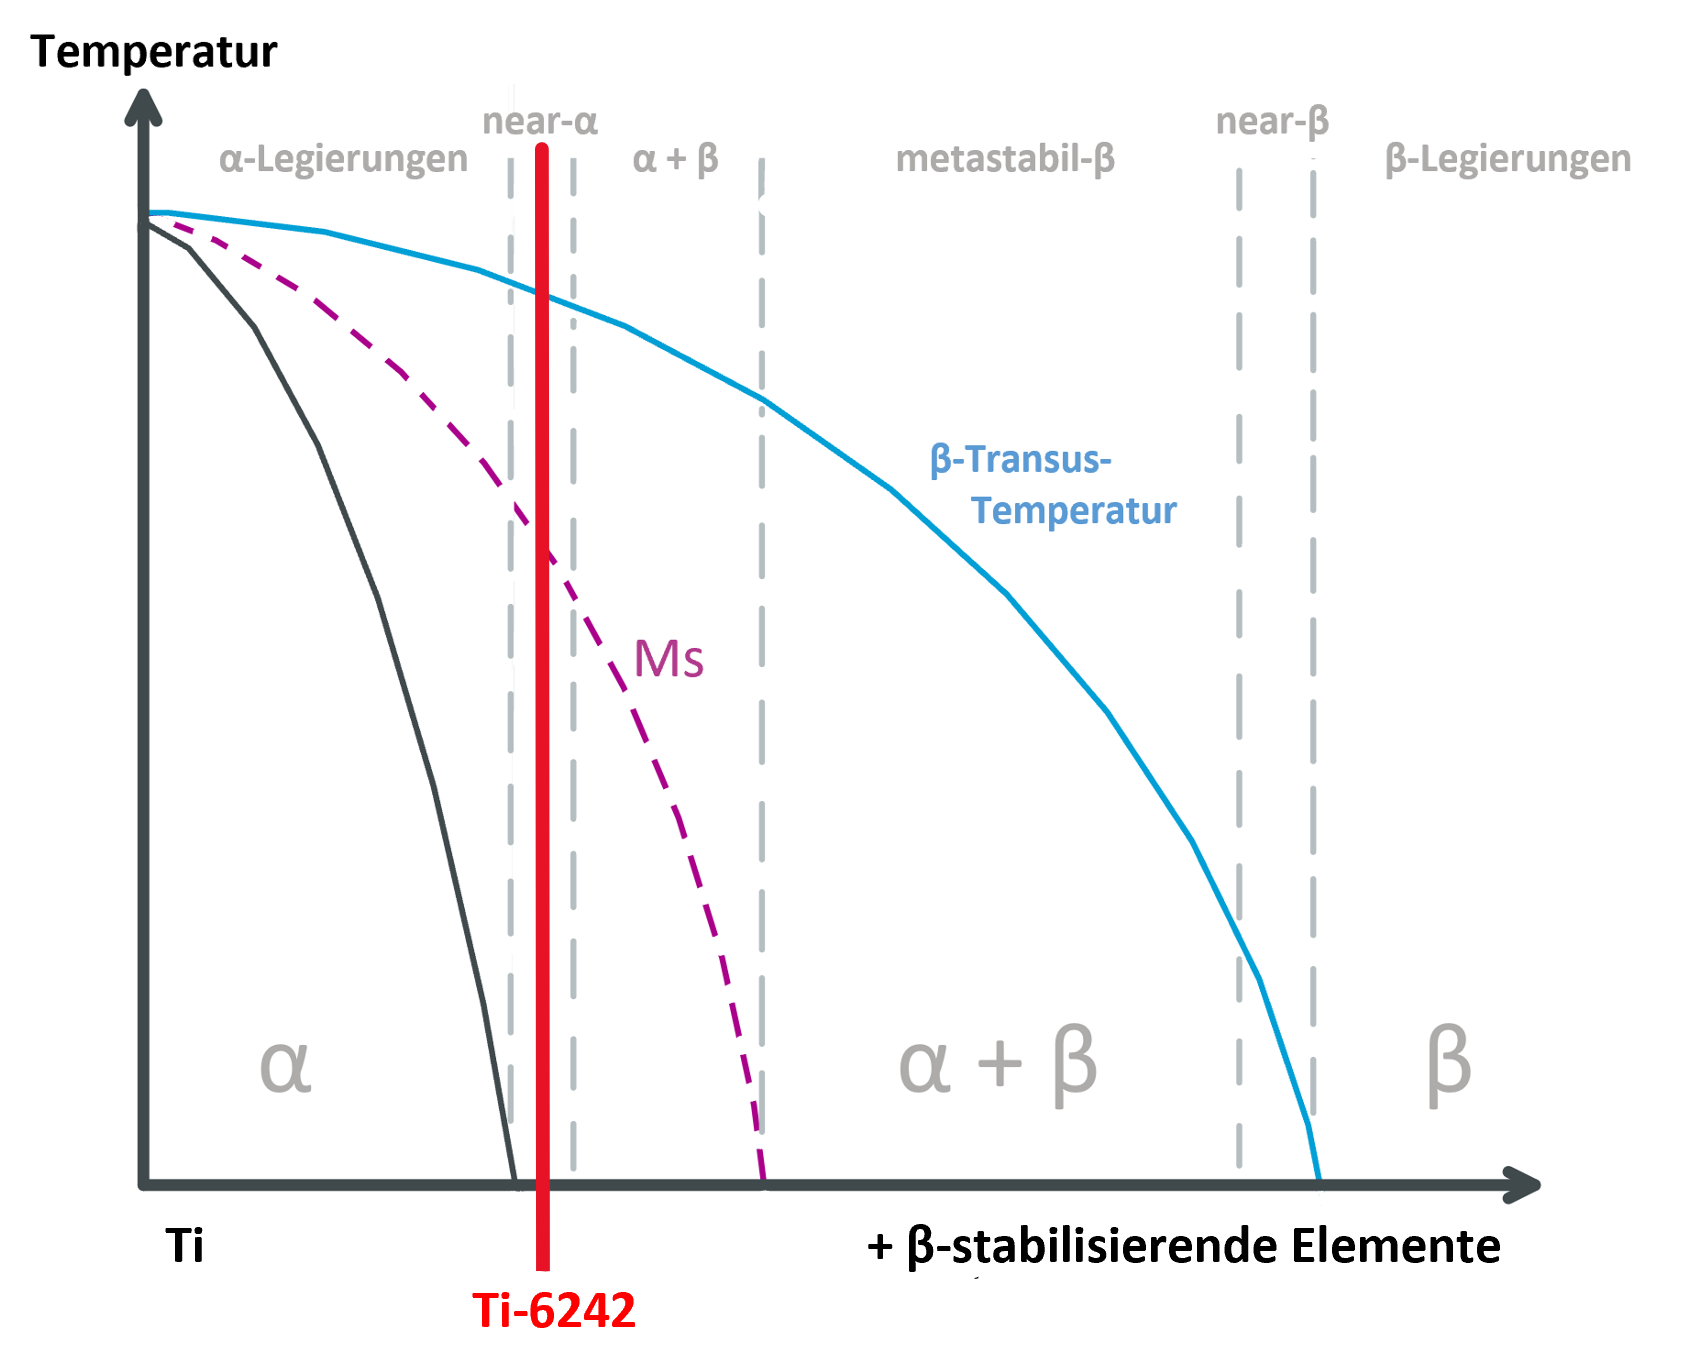
\includegraphics[width=0.5\textwidth]{Bilder/Phasendiagram}
	\caption{Phasendiagramm [Titanium Technical guide]}
\end{figure}





\begin{table}[H]
	\centering	
	\begin{tabular}{|l |c |c|}
		\hline
		\centering
		\hspace{20ex}Elements \hspace{20ex} & Min \%Gwt. & Max \%Gwt.\\
		\hline
		Aluminium&5,5&6,5\\
		Tin&1.80&2.20\\
		Zirconium&3.60&4.40\\
		Molybdenum&1.80&2.20\\
		Silicon &0.06&0.13\\
		Iron&-&0.25\\
		Oxygen&-&0.15\\
		Carbon&	-&	0.05\\
		Nitrogen&-&0.03\\
		Hydrogen&-&0.0125\\
		
		Titanium &&Remainder\\
		\hline
	\end{tabular}
	\caption{Zusammensetzung von Ti-6242 [Titanium : Technical guide]}
\end{table}


Die Ti6242S ist eine Optimierung von Ti6242, die erst 1974 entwickelt wurde. Dieser wurde zusätzlich Silizium in kleinen Mengen zulegiert, um die Resistenz gegen Kriechen vor allem bei hohen Temperaturen durch die Bildung von Siliziden zu erhöhen.  [Immanuel Freiherr von Thungen]. 

Verzeichnis : [Immanuel Freiherr von Thungen] - Immanuel Freiherr von Thungen. Effet dwell: relation microstructure-microtexture-propriétés mécaniquesdel’alliagedetitaneTi6242. Autre. ISAE-ENSMAEcoleNationaleSupérieuredeMécanique et d’Aérotechique - Poitiers, 2016. Français. NNT: 2016ESMA0027 .  tel-01486574
\subsubsection{Kristallstruktur}

Ti6242 wird klassischerweise in der bimodalen oder Duplex-Struktur eingesetzt die nach einer typischen Wärmebehandlung , erklärt in Abbildung \ref{WB} , erreicht  werden kann.

\begin{figure}[H]
	
	\centering
	
	{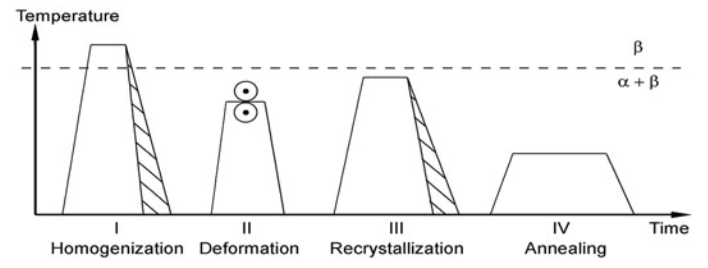
\includegraphics[width=1\textwidth]{Bilder/WB}}			
	\caption{Schematic processing route for bi-modal microstructures ofa+btitanium alloys )}
	\label{WB}
\end{figure}
nach DEFORMATION !!!Bei der Erwärmung von Raumtemperatur  auf T1 < Beta-trans wandelt sich ein Anteil von der Alpha-Phase in Beta um. Nach 1-2h werden die Werkstücke wieder auf Raumtemperatur luftgekühlt.
Dabei wandelt sich das Beta in Beta + Alpha Lamellen um. (Photovom Gefüge ...).
Als letzte Wärmebehandlung wird normalerweise  Ti6242 für  8 h  bei 595 °C angelassen. (Aerospace Materials and Material Technologies )
Wärmebehandlungen von Ti6242 und deren Einflussen werden in den nächsten Kapiteln noch genauer diskutiert.


\subsubsection{ Physikalische und mechanische Eigenschaften }

Die Tabelle in Abbildung ... fasst ein paar physikalische Kennwerte vom Ti-6242 zusammen.

\begin{table}[H]
	\centering	
	\begin{tabular}{|l |c |c|c |c|}
		\hline
		\centering
		Thickness[mm] & Tensile strength [MPa] & Yield strengh [MPa] & Elongation[\%]& Reduction in Area [\%]. \\
		\hline
		25-50&1000&930&14&33\\
		102&1000&930&12&30\\
		205&1035&940&12&28\\
		330&1000&825&11&21\\
		
		\hline
	\end{tabular}
	\caption{Physikalische Kennwerte von Ti6242 : ???]}
\end{table}


Die mechanischen Eigenschaften von Titanlegierungen, wie bereits im ersten Kapitel erklärt wurde, hängen hauptsächlich von den verschiedenen Wärmebehandlungen ab, die die Gefügestruktur des Werkstoffes  verändern und so auch sein thermomechanisches Verhalten.
Als eine Near-Alpha Titan Legierung, ist Ti6242 zum größten Teil Alpha (90-95\%). Da die Diffusionsrate bei Beta-Strukturen höher ist als bei Alpha-Strukturen weist Ti6242 eine bessere Stabilität bei höheren Temperaturen auf + Temperatur Bereich !!!!. (Aerospace Materials and Material Technologies ) 

Die Alpha-Beta Transformationstemperatur von Ti-6242 liegt bei 995°C +- 15°C. Die Abweichung hängt  von den Anteilen der verschiedenen Legierungselementen ab. Wie bereits im ersten Kapitel beschrieben wurde, stabilisieren  Al, O , N und C die Alpha Phase und erhöhen im Gegensatz zu Mo die Beta-transus Temperatur.
Aufgrund des niedrigen Mo-Gehalts von Ti6242 liegt ihre Betat-trans-Temperatur oberhalb der von Reinem Titan, die bei 882 +- 2°C liegt.


\begin{table}[H]
	\small
	\tabcolsep=0.11cm
	\centering	
	\begin{tabular}{|l |c |c|c |c|}
		\hline
		\centering
		Thickness[mm] & Tensile strength [MPa] & Yield strengh [MPa] & Elongation[\%]& Reduction in Area [\%]. \\
		\hline
		25-50&1000&930&14&33\\
		102&1000&930&12&30\\
		205&1035&940&12&28\\
		330&1000&825&11&21\\
		
		\hline
	\end{tabular}
	\caption{Elatische Eigenschaften bei Raumtemperatur von Ti6242Si (Annealed 1h 954°C/AC + 8h/600°C/AC )  [Titanium : Technical guide]}
	\label{Mecprop}
\end{table}






%	Für den Einsatz in der Luftfahrt sind aber auch spezielle mechanische  Eigenschaften wie zB eine hohe Festigkeit und Duktilität, eine hohe Kriech- und Korrosionsbeständigkeit bei relativ hohe Temperaturen gesucht.   

Alle sekundären Fertigungsverfahren, die für die Herstellung von Bauteilen erforderlich sind   wie zB. Biegen, Fräsen und Schweißen können Eigenschaften von Titan oder Titanlegierungen stark beeinflussen  und müssen daher mitberücksichtigt werden.




\subsubsection{Verwendung}
Für den Oben genanten Eigenschaften, die der Ti6242/Ti6242S bezeichnen, werden diese Legierungen hauptsächlich in der Luftfahrt eingesetzt. Vor allem bei rotierenden Teilen im Triebwerk, wo  hohe Kriechbeständigkeit, Ermüdungsresistenz  neben eine hohe metallurgische Stabilität bei hohen Temperaturen erforderlich sind. 





Diese Legierung wird aufgrund ihres guten Festigkeit-Gewichtsverhältnisses und ihrer  Stabilität bei hohen Temperaturen (538°C - 595 °C) hauptsächlich in der Luft- und Raumfahrt  verwendet.\newline
Ti6242 wird z.B. in der Herstellung von Hochdruckverdichtern, Turbinenschaufeln und Nachbrennern verwendet, wo neben den oben erwähnten Eigenschaften auch die Korrosionsbeständigkeit bei hohen Temperaturen erforderlich ist. \newline



\begin{figure}[H]
	\centering
	\subfloat[Compressor spoolfor GE CF6 class engine using inertia welding toconnect the individual stages:front (smaller)five stages: Ti–6Al–4V; rear two stages:Ti-6242 ]
	{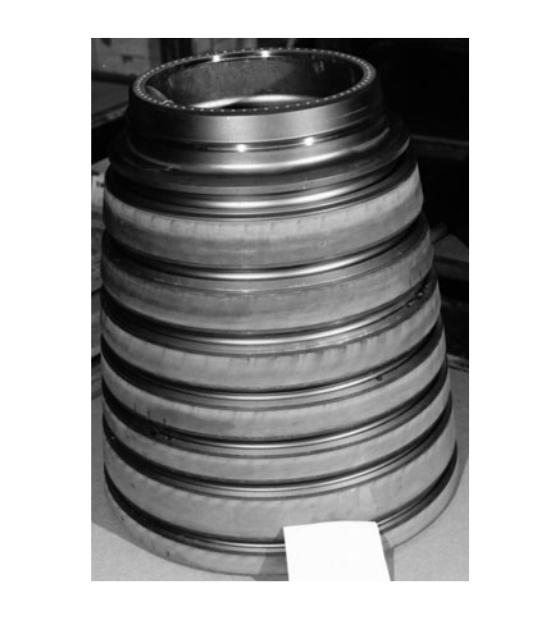
\includegraphics[width=0.5\textwidth]{Bilder/Compressor spool}}
	\hspace{5ex}
	\subfloat[Impeller used in asmall engine for regional jets, diameter 35 cm. The alloy is Ti-6242 with a bi-modalmicrostructure]
	{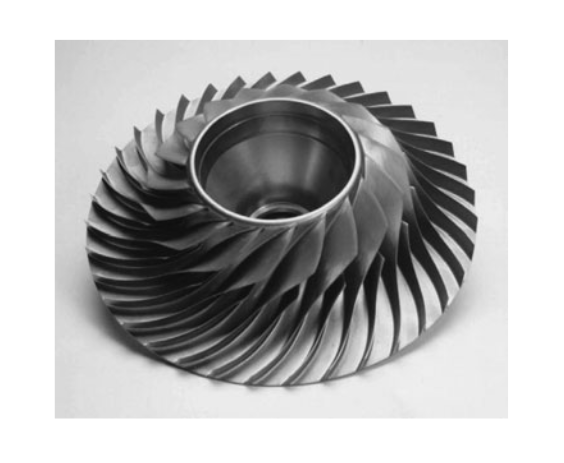
\includegraphics[width=0.5\textwidth]{Bilder/Impeller}}
	\caption{Beispiele von Einsatzbereiche von Ti-6242 (Aerospace Materials and Material Technologies )}
	
\end{figure}


